\documentclass[]{article}

\usepackage[utf8]{inputenc}
\usepackage[paperheight=1.5in,paperwidth=2.1in,margin=0in]{geometry}
\usepackage{tikz}
\usetikzlibrary{shapes,arrows,automata,calc}
\usepackage{color}

\usepackage{booktabs}  % nicer table borders 

\begin{document}

%\clearpage
%\thispagestyle{empty}

\tiny{
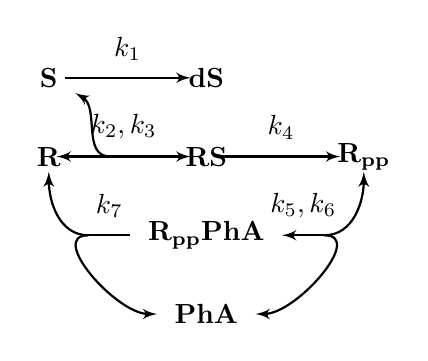
\begin{tikzpicture}[auto, outer sep=3pt, node distance=0cm,>=latex']

\node  at (-8.1, 8) (S) {$\bf S$};
\node  at (-6.1, 8) (dS) {$\bf dS$};
\draw [->, thick] ($(S)+(0.2,0)$) to node {$k_1$} ($(dS)+(-0.2,0)$);

\node  at (-8.1, 7) (R) {$\bf R$};
\node  at (-6.1, 7) (RS) {$\bf RS$};
\node  at ($(R)!0.5!(RS)$) (RRS) {};
\draw [<->, thick] ($(R)+(+.1,0)$) to node {$k_2, k_3$} ($(RS)+(-0.2, 0)$);
\draw [<-, thick] (S) edge[in=180, out=330] (RRS);
%\node  at (-3.8, 7.8) (X3) {$k_4^{cat},K_4m$};

\node at (-4.1, 7) (Rpp) {$\bf R_{pp}$};
\draw [->, thick] ($(RS)+(+.2,0)$) to node {$k_4$} ($(Rpp)+(-0.3, 0)$);


\node at (-6.1, 6) (RppPha) {$\bf R_{pp}PhA$};
\node at (-7.6, 6) (LeftRppPha) {};
\node at (-4.6, 6) (RightRppPha) {};
\draw [<-, thick] ($(Rpp)+(0, -0.2)$) edge[out=270, in=0] ($(RightRppPha)$);
\draw [<-, thick] ($(R)+(0, -0.2)$) edge[out=270, in=180] ($(LeftRppPha)$);
\draw [->, thick] ($(RightRppPha)$) to node[above] {$k_5, k_6$} (RppPha);
\draw [-, thick] ($(LeftRppPha)$) to node[above] {$k_7$} (RppPha);

\node at (-6.1, 5) (Pha) {$\bf PhA$};
\draw [<-, thick] (Pha) edge[in=0, out=0] (RightRppPha.center);
\draw [<-, thick] (Pha) edge[in=180, out=180] (LeftRppPha.center);



\end{tikzpicture} 
}

\end{document}

